\documentclass[a4paper]{report}

\usepackage{hyperref}
\hypersetup{
    colorlinks,
    citecolor=black,
    filecolor=black,
    linkcolor=black,
    urlcolor=black
}

\usepackage{url}
\usepackage{amsmath}
\usepackage{verbatim}   		% Useful for program listings
\usepackage[T1]{fontenc}       	% For Swedish characters ÅÄÖ etc.
\usepackage[utf8]{inputenc}
% \usepackage[swedish]{babel} % For Swedish hyphenation
\usepackage{fancyvrb}           	% For lists with tabulators
\fvset{tabsize=4}              	 	% Tabulator size
\fvset{fontsize=\small}         	% List font size
\usepackage{graphicx}		% Imports the graphicx package, useful for images
% \usepackage{}
% \makeatletter\@addtoreset{chapter}{part}\makeatother% % Makes chapter numbering reset after each part
\usepackage{listingsutf8}
\lstset{
  basicstyle=\scriptsize\ttfamily,
  language=C,
	extendedchars=true,
  inputencoding=utf8,
  commentstyle=\color{black},
	gobble=12
}

\title{Dragonfly Quadrotor UAV \\ Flight Control Board}
\author{Nina Khayyami \\ Adam Steineck \\ Daniel Stenberg }

\date{\today}         			% Sets date on first page

\begin{document}                	% Start of document

\maketitle                      		% Prints the title defined above with \title, \author and \date

\newpage

\tableofcontents				% Insert table of contents

\newpage

\chapter{List of Abbreviations}

\chapter{Introduction}

The \emph{Dragonfly} project is an internal competence enhancement project for ÅF employees. The goal is to combine technology, competence and experience from various engineering fields in order to construct a highly advanced quadrotor UAV system. The focus of the Flight Control Board development deals with low-level maneuvering of the aircraft, calculating motor command based on a feedback control system. Some of the major technologies deployed to attain this are control theory, electronics and software development.

An early CAD rendeded image of the Dragonfly quadrotor concept can be viewed in Figure \ref{fig:quadrendered1}.

\begin{figure}[h]
    \centering
    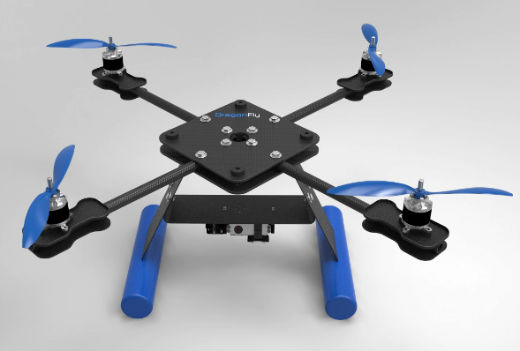
\includegraphics[scale=0.4]{images/quad_concept1_rendered.jpg}
    \caption{Rendered image of one of the first quadrotor designs concepts}
    \label{fig:quadrendered1}
\end{figure}

%
% THEORY PART STARTS HERE!
%
\part{Theory}

\chapter{Introduction}
This part concerns the physical, mathematical and control system theory essential to understand the quadrotor system sufficiently to control its flight. The flight theory presents a rigid-body dynamical model of the quadrotor flight as well as representation of coordinate systems suitable to present aircraft states such as position, attitude and velocity. Aerodynamic effects on this system is also presented and discussed. For the control part, the problem of controlling the aircraft is split in to two distinct parts - estimating the current states and controlling the system to achieve desired states.

\chapter{System Description}

	\section{Coordinate System Representation}
World-frame and body-frame coordinate systems. Euler angles and rotation matrices. Transformations between coordinate frames.

	\section{Flight Dynamics}

	\section{BLDC Motor Theory}
	\label{sec:BLDCMotorTheory}
Brushless DC electric motor (BLDC motors, BL motors) also known as electronically commutated motors (ECMs, EC motors) are synchronous motors that are powered by a DC electric source via an integrated inverter/switching power supply, which produces an AC electric signal to drive the motor. In this context, AC, alternating current, does not imply a sinusoidal waveform, but rather a bi-directional current with no restriction on waveform. Additional sensors and electronics control the inverter output amplitude and waveform (and therefore percent of DC bus usage/efficiency) and frequency (i.e. rotor speed).

Electrical motors are based on interaction between two magnetic fields, one produced by a permanent magnet and one by current flowing in the motor windings. The fields produce a torque which drives the rotor. During rotation, the current in the winding is commutated (reversed) to obtain a continuous torque.

The BLM motors used for this project have an “outrunner” architecture, which means that the permamagnet rotor lies outside the winding stator. The windings are separated into several coils energized cyclically (AC current) by an electronic speed controller (ESC) to achieve rotor rotation.

	\section{Radio Control Theory}

	\section{Sensor Theory}

		\subsection{Microelectromechanical Systems (MEMS) Sensors}

		\subsection{Gyroscope}

		\subsection{Accelerometer}

		\subsection{Magnetometer}

\chapter{State Estimation Theory}
The state vector for the attitude is the attitude angle and the angular rate bias. The latter is due to gyroscope having a drift in its measured angular velocity, that is, taking a number of samples and averaging the value and using this as an offset.
	\section{Attitude Estimation}
		Step 1: Predict the estimated states $\hat{x}_{k|k-1}$
		\begin{equation}
		\hat{x}_{k|k-1}=A\hat{x}_{k-1|k-1}+Bu_{k}
		\end{equation}

		\begin{equation}
		\left[
      		\begin{array}{c}
      		\hat{\theta}\\
		\hat{\dot{\theta}}_{b}
      		\end{array} \right]_{k|k-1}
		=
		\left[
		\begin{array}{c c}
		1 & - \Delta T\\
		0 & 1
		\end{array} \right]
		\left[
		\begin{array}{c}
		\hat{\theta}\\
		\hat{\dot{\theta}}_{b}
		\end{array} \right]_{k-1|k-1}
		+
		\left[
		\begin{array}{c}
		\Delta T\\
		0
		\end{array} \right]
		\dot{\theta}_{gyro, k}\\
		\end{equation}
		\begin{equation*}
		z_{k}=
		\left[
		\begin{array}{c c}
		1 & 0
		\end{array} \right]
		\left[
		\begin{array}{c}
		\theta\\
		\dot{\theta}_{b}
		\end{array} \right]_{k|k-1}
		\end{equation*}
    In pseudo code:
    \begin{lstlisting}[frame=single]
		predictAngle = angle + dt*gyroRate - dt*bias;
		//gyroRate is the rate from the gyroscope
		predictBias = bias;
		\end{lstlisting}

		Step 2: Predict the error covariance matrix $P_{k|k-1}$,
		\begin{equation}
		P_{k|k-1}=AP_{k-1|k-1}A^{T}+Q
		\end{equation}

		where $Q$ is the process noise covariance matrix.

		\begin{equation*}
		\left[
		\begin{array}{c c}
		P_{00}	&	P_{01}\\
		P_{10}	&	P_{11}
		\end{array} \right]_{k|k-1}
		=
		\left[
		\begin{array}{c c}
		1 & - \Delta T\\
		0 & 1
		\end{array} \right]
		\left[
		\begin{array}{c c}
		P_{00}	&	P_{01}\\
		P_{10}	&	P_{11}
		\end{array} \right]_{k-1|k-1}
		\left[
		\begin{array}{c c}
		1	&	0\\
		- \Delta T & 1
		\end{array} \right]
		+
		\end{equation*}
		\begin{equation}
		+
		\left[
		\begin{array}{c c}
		\sigma(\dot{\theta}_{gyro})\cdot\Delta T^{2}	&	0\\
		0	&	 \sigma(\dot{\theta_{b}})
		\end{array} \right]
		\end{equation}
    In pseudo code:
		\begin{lstlisting}[frame=single]
		P[0][0] += dt*(dt*P[1][1] - P[0][1] - P[1][0] + Q1);
		P[0][1] -= dt*P[1][1];
		P[1][0] -= dt*P[1][1];
		P[1][1] += dt*Q2;
		\end{lstlisting}
		Step 3: Now calculate the difference $\tilde{y}_{k}$ between the predicted state $\hat{x}_{k|k-1}$ and the measurement $z_{k}$
		\begin{equation}
		z_{k}=H\hat{x}_{k|k-1}
		\end{equation}
		\begin{equation}
		\tilde{y}_{k}=z_{k}-H\hat{x}_{k|k-1}
		\end{equation}
		The extraction matrix $H$ matrix defines what sensor readings we would get under the conditions that our $\hat{x}$ was perfectly estimated and our sensors delivered perfect values.\footnote{See  \url{https://www.udacity.com/wiki/cs373/kalman-filter-matrices}}
		
		\begin{equation}
		\tilde{y}_{k}=z_{k}-\left[
		\begin{array}{c c}
		1	&	0
		\end{array} \right]
		\left[
		\begin{array}{c}
		\theta \\
		\dot{\theta}_{b}
		\end{array} \right]_{k|k-1}
		\end{equation}
    In pseudo code:
		\begin{lstlisting}[frame=single]
		y = sensorAngle - predictAngle;
		//sensorAngle is the angle computed from sensor values
		\end{lstlisting}
		Step 4: Calculate the innovation covariance matrix $S_{k}$
		\begin{equation}
		S_{k}=HP_{k|k-1}H^{T}+R
		\end{equation}

		where $R$ is the measurement noise covariance matrix.

		\begin{equation}
		S_{k}=
		\left[
		\begin{array}{c c}
		1	&	0
		\end{array} \right]
		\left[
		\begin{array}{c c}
		P_{00}	&	P_{01}\\
		P_{10}	&	P_{11}
		\end{array} \right]_{k|k-1}
		\left[
		\begin{array}{c}
		1\\
		0
		\end{array} \right]
		+ \sigma(\theta_{acc})
		\end{equation}

		where
		\begin{equation*}
		\theta_{acc}=\arctan{\left(\frac{a_{y}}{a_{z}}\right)}
		 \end{equation*}
    In pseudo code:
		\begin{lstlisting}[frame=single]
		S = P[0][0] + R;
		\end{lstlisting}
		Step 5: Calculate the Kalman gain $K_{k}$
		\begin{equation}
		K_{k}=P_{k|k-1}H^{T}S^{-1}_{k}
		\end{equation}

		\begin{equation}
		\left[
		\begin{array}{c}
		K_{0}\\
		K_{1}
		\end{array} \right]_{k}
		=
		\left[
		\begin{array}{c c}
		P_{00}	&	P_{01}\\
		P_{10}	&	P_{11}
		\end{array}  \right]_{k|k-1}
		\left[
		\begin{array}{c}
		1\\
		0
		\end{array} \right]
		S^{-1}_{k}
		\end{equation}
    In pseudo code:
		\begin{lstlisting}[frame=single]
		K[0] = P[0][0] / S;
		K[1] = P[1][0] / S;
		\end{lstlisting}
		Step 6: Update the state prediction $\hat{x}_{k|k-1}$ to  $\hat{x}_{k|k}$
		\begin{equation}
		\hat{x}_{k|k}=\hat{x}_{k|k-1}+K_{k}\tilde{y}_{k}
		\end{equation}

		\begin{equation}
		\left[
		\begin{array}{c}
		\theta\\
		\dot{\theta}_{b}
		\end{array} \right]_{k|k}
		=
		\left[
		\begin{array}{c}
		\theta\\
		\dot{\theta}_{b}
		\end{array} \right]_{k|k-1}
		+
		\left[
		\begin{array}{c}
		K_{0}\\
		K_{1}
		\end{array} \right]_{k}
		\tilde{y}_{k}
		\end{equation}
    In pseudo code:
		\begin{lstlisting}[frame=single]
		correctAngle = predictAngle + K[0]*y;
		correctBias = predictBias + K[1]*y;
		\end{lstlisting}
		Step 7: Update the error covariance matrix prediction $P_{k|k-1}$ to $P_{k|k}$
		\begin{equation}
		P_{k|k}=(I-K_{k}H)P_{k|k-1}
		\end{equation}

		\begin{equation}
		\left[
		\begin{array}{c c}
		P_{00}	&	P_{01}\\
		P_{10}	&	P_{11}
		\end{array} \right]_{k|k}
		=
		\left(
		\left[
		\begin{array}{c c}
		1	&	0\\
		0	&	1
		\end{array} \right]
		-
		\left[
		\begin{array}{c}
		K_{0}\\
		K_{1}
		\end{array} \right]_{k}
		\left[
		\begin{array}{c c}
		1	&	0
		\end{array} \right]
		\right)
		\left[
		\begin{array}{c c}
		P_{00}	&	P_{01}\\
		P_{10}	&	P_{11}
		\end{array} \right]_{k|k-1}
		\end{equation}
    In pseudo code:
		\begin{lstlisting}[frame=single]
		float P00_tmp = P[0][0];
		float P01_tmp = P[0][1];

		P[0][0] -= K[0]*P00_tmp;
		P[0][1] -= K[0]*P01_tmp;
		P[1][0] -= K[0]*P00_tmp;
		P[1][1] -= K[0]*P01_tmp;
		\end{lstlisting}

	\section{Velocity Estimation}
	Kalman filters are used to estimate the angles, $\theta_{k}$, and in order to find the angular velocity, $\dot{\theta}_{k}$, we can calculate the derivative of the angle.
	\begin{equation}
	\label{thetaDot}
	\dot{\theta}_{k}=\frac{\theta_{k}-\theta_{k-1}}{\Delta T}
	\end{equation}

	Question: Is the $\Delta T$ in the above equation the same $\Delta T$ as in the attitude estimation equations? If they differ, I think that $\Delta T$ that is used in the Kalman filter is the sample rate for the sensor values, and $\Delta T$ in equation (\ref{thetaDot}) is the period for a Kalman filter iteration.

\chapter{Flight Control Theory}

	\section{Control Design Overview}

Figure \ref{fig:controloverview} shows an overview of the control problem.

\begin{figure}[h]
    \centering
    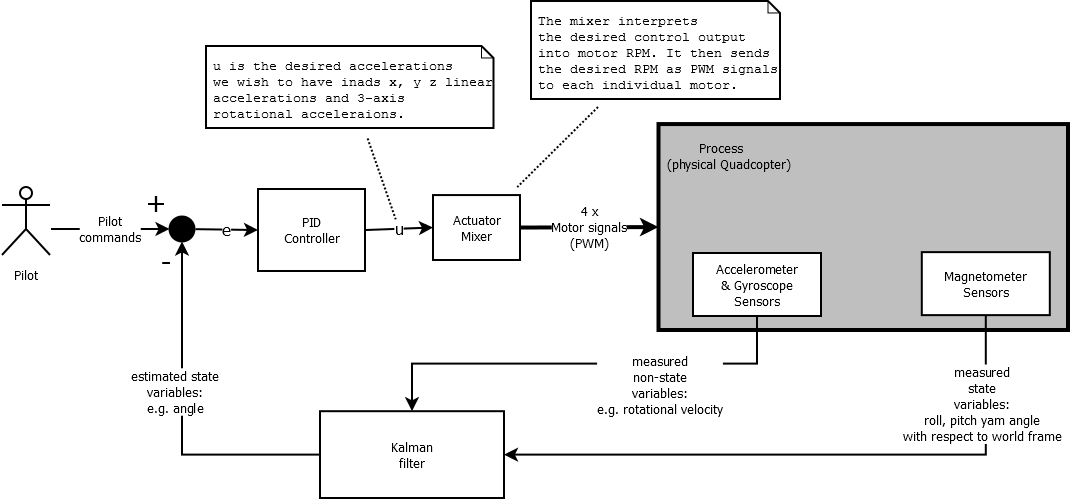
\includegraphics[scale=0.3]{images/ControlDiagram.png}
    \caption{Control overview diagram}
    \label{fig:controloverview}
\end{figure}

	\section{PID Control}

		\subsection{The algorithm}
The PID control strategy is one of the most commonly used control algorithms. It consists of three parts that each contribute to the control signal; Proportional (P), Integral (I) and Derivative (D). The equation for the PID algorithms is presented in (\ref{PID_classic}), where $u(t)$ is the control signal and $e(t) = y_{ref}(t) - y(t)$ is the control error. This is the classical representation without any modifications. When used in practice, some alterations are typically made to address some practical issues and increase performance in a real-world environment. For one, it needs to be discretized so that a digital computer may generate control signals, but there are numerous other modifications to consider.

\begin{equation}
u(t) = K \bigg( e(t) + \dfrac{1}{T_i} \int_{0}^{\infty}  e(t) dt + T_d \dfrac{d}{dt} e(t) \bigg)
\label{PID_classic}
\end{equation}

When tuning the algorithm (\ref{PID_classic}), a set of parameters $K$, $T_i$, $T_d$ are selected by, for example, pole placement, step response analysis or frequency diagram design.

	\subsection{Practical modifications}
To ensure performance in a real-world environment, a number of modifications are typically made to address the following issues:

\begin{itemize}
\item High-frequency noise
\item Integrator wind-up due to saturation
\item Transfer between control parameters and modes
\end{itemize}

Along with this, a few other parameters are introduced enable more possibilities to achieve desired performance.

	\subsection{Discretization}
To run the algorithms on a digital system, the equation needs to be discretized. This is often achieved using a finite-step approximation such as backward and forward difference or Tustin approximation.

	\section{Attitude Control}

	\section{Velocity Control}

\chapter{Sensor Calibration Algorithms}

	\section{Gauss-Newton Optimization}

	\section{Magnetometer calibration}

	\section{Accelerometer calibration}

%
% IMPLEMENTATION PART STARTS HERE!
%
\part{Implementation}

\chapter{Introduction}
In this part, the implementation of the flight control system is presented and discussed. It concerns documentation of both electronic and software design choices. The heart of the flight control system is the \emph{Flight Control Board} (FCB) program, running on an STM32F303VC microcontroller attached to an STM32F3Discovery board featuring on-board sensors, debug interface and more. The program is mainly written in C code and executes code to, among other things, control and actuate the motors, read from the sensors and an RC receiver and estimate the flight states.

\chapter{Hardware}

	\section{Flight Control Board - STM32F3Discovery}
The STM32F3Discovery is an evaluation board provided by STMicroelectronics. It features an STM32F303VCT6 microprocessor based on the ARM Cortex-M4 core. For evaluation purposes, the board has been fitted with accelerometer, magnetometer and gyroscope sensors, an on-board ST-Link/V2 debugger/programmer, various LED:s, extension headers for all I/O pins and more.

\begin{itemize}
  \item CPU speed: $72$ MHz
  \item ROM: $256$ kB Flash
  \item RAM: $48$ kB ($40$ kB SRAM, $8$ kB CCM)
  \item I/O pins: LQFP100 pin package with pins attached to extension header
  \item On-board ST-LINK/V2 programming and debugging device
  \item Power supply: From USB bus or from an external $3$ $V$ or $5$ $V$ supply voltage
  \item L3GD20 MEMS gyroscope
  \item LSM303DLHC MEMS accelerometer and magnetometer
  \item 10 LEDs
  \item Two pushbuttons
  \item USB USER Mini-B connector
\end{itemize}

Figure \ref{fig:stm32f3busmatrix} shows the microcontroller internal bus matrix, connecting the core to the MCU peripherals.

\begin{figure}[h]
    \centering
    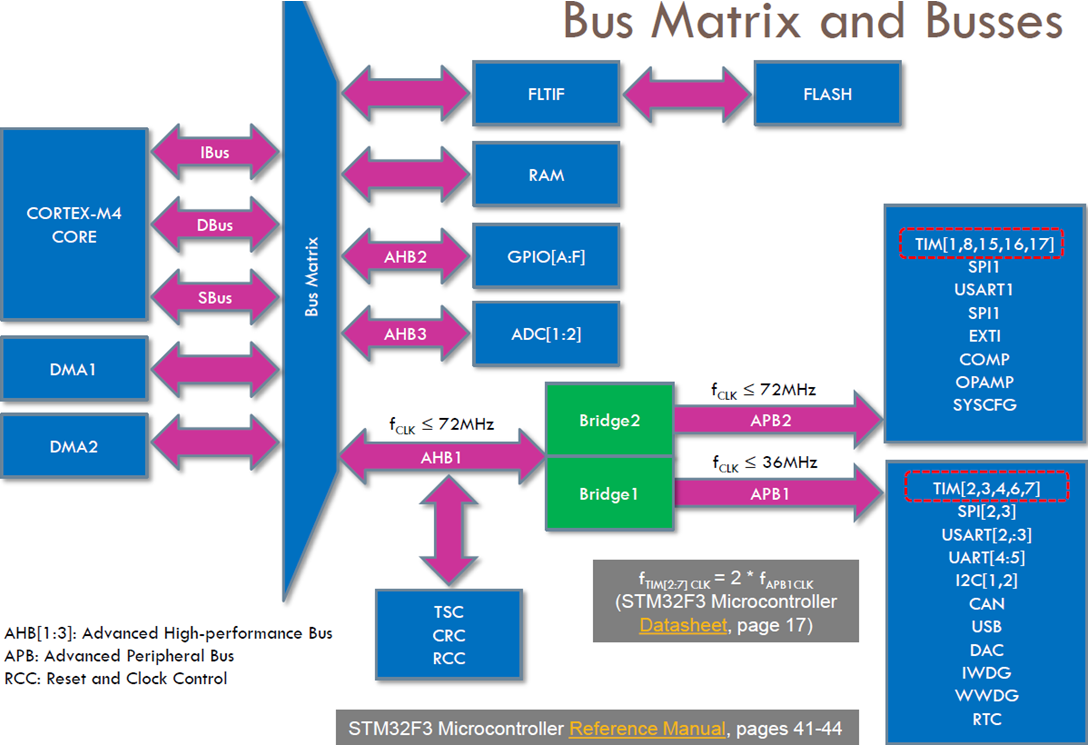
\includegraphics[scale=0.4]{images/stm32_busmatrix.png}
    \caption{STM32F3 bux matrix}
    \label{fig:stm32f3busmatrix}
\end{figure}

	\section{T-Motor U3 BLDC Motors}
The motors of choice for the Dragonfly are of the type \emph{T-motor U3}, which are sensorless (no built-in Hall sensor) brushless motors, designed to deliver high performance and reliability. According to the manufacturer, they are highly resistant to dirt and water. There are several benefits of using brushless motors instead of traditional DC motors, including longer life-time (due to no brushes that become worn out), less noisy operation and more efficient cooling.

The T-motor U3 motors have 12 stator coils and 14 rotor magnets. The motor theory was earlier presented in Section \ref{sec:BLDCMotorTheory}.

\begin{itemize}
  \item Motor velocity constant: $700$ $rpm/V$
  \item Stator-pole configuration: $12N-14P$
  \item Dimensions: Diameter: $41.80$ $mm$, Height: $30.75$ $mm$
  \item Weight: $97$ $g$
  \item Idle current: $0.5$ $A$
  \item Recommended number of battery cells (LiPo): $3-4S$
  \item Max continuous current ($180$ $s$): $25$ $A$
  \item Max continuous power ($180$ $s$): $400$ $W$
  \item Max current efficiency: ($4-10$ $A$) $>82$ \%
  \item Internal resistance: $50$ $m\Omega$
\end{itemize}

\begin{figure}[h]
    \centering
    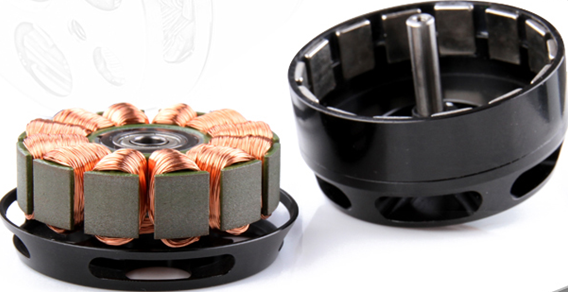
\includegraphics[scale=0.6]{images/tmotoru3open.png}
    \caption{T-Motor U3 BLDC motors}
    \label{fig:tmotoru3open}
\end{figure}

The motor and propeller manufacturer, T-motors, provides some information on the actuation characteristics in Table \ref{table:motorManufacturerData}. The values were obtained with an operating temperature of $43^{\circ}$ $C$ with 11x3.7 inch T-motors carbon fibre propellers attached to the motor shaft.

\begin{table}
\begin{tabular}{ |c|c|c|c|c|c| }
\hline
\textbf{Throttle} & \textbf{Current} & \textbf{Power} & \textbf{Thrust} & \textbf{Speed} & \textbf{Efficiency} \\
\textbf{\%} & \textbf{[$A$]} & \textbf{[$W$]} & \textbf{[$g$]} & \textbf{[$rpm$]} & \textbf{[$g/W$]} \\
\hline
$50$ & $3.2$ & $48$ & $460$ & $5300$ & $9.58$ \\
$65$ & $6.0$ & $87$ & $710$ & $6500$ & $8.16$ \\
$75$ & $8.2$ & $120$ & $870$ & $7500$ & $7.25$ \\
$85$ & $11.0$ & $160$ & $1080$ & $8200$ & $6.75$ \\
$100$ & $13.0$ & $193$ & $1230$ & $8700$ & $6.37$ \\
\hline
\end{tabular}
\caption{T-Motor U3 motor with 11x3.7 inch CF propeller data}
\label{table:motorManufacturerData}
\end{table}

	\section{T-Motor ESC30A Electronic Speed Controllers}
Motor speed control is achieved using ESCs, which cyclically shift the coils’ current by applying a three-phase alternating-current. So the motors themselves are really AC motors, although driven by a DC power source (battery).

The battery drain is determined using MOSFET transistors. By feeding an ESC with a pulse-width modulated (PWM) signal, battery power is switched on and off rapidly for periods decided by the PWM duty cycle. Since this is done at a sufficiently high frequency, the supplied current (which is modulated to AC) “seen” by the motors can be approximated to the mean battery drain. So, the higher the duty cycle the more battery drain and the higher larger electromagnetic torque generated in motor.

The ESCs of choice for this project is the \emph{T-Motor ESC30A}, shown in Figure \ref{fig:esc_tmotor}. It takes a PWM input signal up to $400$ $Hz$ to drive the motors. Normally in RC applications, a $1$ $ms$ pulse width indicates $0$ \% throttle, whereas $2$ $ms$ is 100 \% throttle (with $50$ \% being approx. $1.5$ $ms$). The ESCs feature BEC (Battery eliminator circuit), which outputs a low-power $5$ $V$ source useful to power onboard electronics.

\begin{figure}[h]
    \centering
    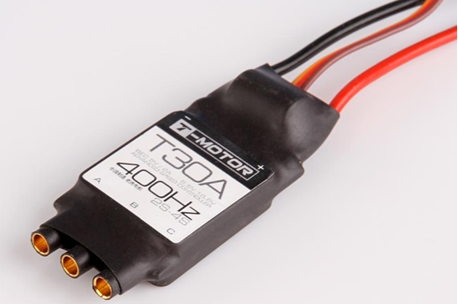
\includegraphics[scale=0.8]{images/esc_tmotor.png}
    \caption{T-Motor ESC30A Electronic Speed Controller}
    \label{fig:esc_tmotor}
\end{figure}

\begin{itemize}
  \item Output: Continuous 30A, Burst 40A up to 10 Secs.
  \item Input: 2-4 cells lithium battery or 5-12 cells NiCd/NIMh battery.
  \item BEC: $2$ $A$ / $5$ $V$ (Linear mode)
  \item Max speed: $35000$ $rpm$ for BLDC motor
\end{itemize}

	\section{RC Receiver and Transmitter}

The Spektrum AR610 receiver, shown in Figure \ref{fig:ar610}, employs full-range $2.4$ GHz DSMX modulated radio communication. It is capable of reading and outputting up to 6 channels of controller information. The output from each channel consists of a PWM signal with a period of $22$ $ms$ (approx. $45.45$ Hz) with a pulse width between (approx.) $1$ and $2$ ms, depending on controller action. There is also an additional receiver output, used for binding the controller with the receiver. The channels are labeled as follows:

\begin{itemize}
  \item BND/DAT (Bind) - Used only to bind the controller to the receiver with the bind plug (see image). More on this can be found in the controller and/or receiver manuals.
  \item THRO (Throttle) – Typically used to control the altitude actuation.
  \item AILE (Aileron) – Typically used to control the roll actuation.
  \item ELEV (Elevator) – Typically used to control the pitch actuation.
  \item RUDD (Rudder) – Typically used to control the yaw actuation.
  \item GEAR – Open to interpretation
  \item AUX (Auxiliary) - Open to interpretation.
\end{itemize}

\begin{figure}[h]
    \centering
    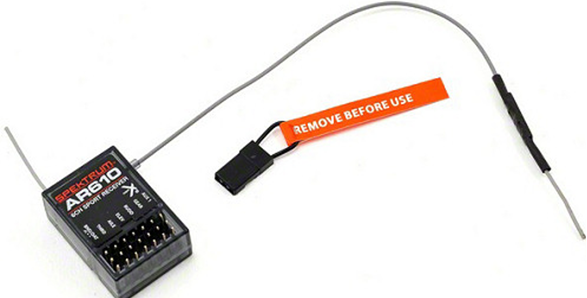
\includegraphics[scale=0.8]{images/ar610.png}
    \caption{Spektrum AR610 receiver}
    \label{fig:ar610}
\end{figure}

The RC transmitter of choice is the Spektrum DX6i, which is a 6-channel transmitter using $2.4$ GHz Spektrum DSMX modulation. In Figure \ref{fig:dx6i_map}, the transmitter's stick and switch mapping and labeling is shown.

\begin{figure}[h]
    \centering
    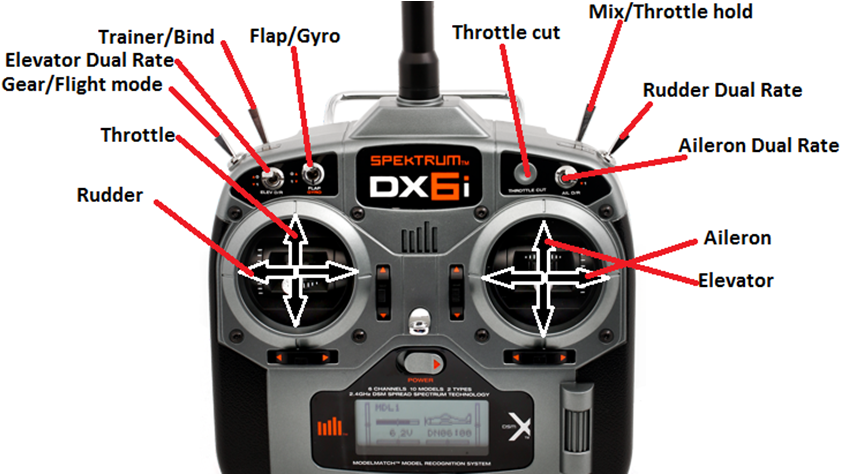
\includegraphics[scale=0.6]{images/dx6i_map.png}
    \caption{Spektrum DX6i RC transmitter labels}
    \label{fig:dx6i_map}
\end{figure}

MCU Timer Input Compare registers are configured and used to read input PWM signals, typically from the RC receiver. They are connected to timer channels to generate interrupts on up and down flanks of PWM pulses (the polarity is reversed after reading each flank).

	\section{Battery}

The battery used is of Lithium polymer type, containing Lithium ions to drive current from the positive to the negative electrode through a closed circuit.

\begin{itemize}
  \item Capacity: $8000$ $mAh$
  \item Voltage: $14.8$ $V$
\end{itemize}

	\section{Sensors}

L3DG20 Gyroscope over SPI. LSM303DLHC over I2C. Orientation with respect to quadrotor coordinate axes.

\chapter{Software}

	\section{System Design Overview}
An overview of the entire software architecture can be viewed in Figure \ref{fig:high-level-sw-arch} below. This document mainly concerns the Flight Control Board development.

\begin{figure}[h]
    \centering
    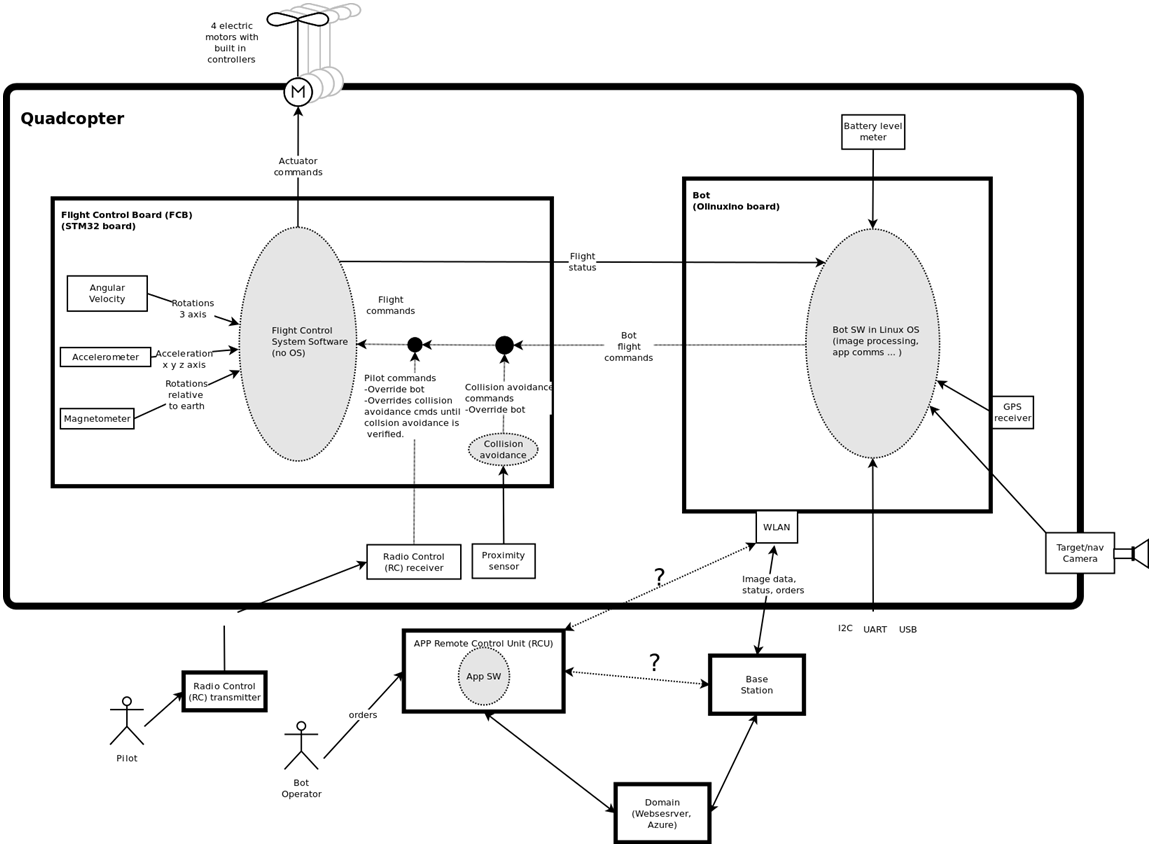
\includegraphics[scale=0.42]{images/high-level-sw-design.png}
    \caption{Overall software architecture}
    \label{fig:high-level-sw-arch}
\end{figure}

As can be viewed in the digram in Figure \ref{fig:fcb-sw-hw-arch}, the Flight Control Board software takes input from a number of sources. Internally, it receives data from the built-in sensors (gyroscope, accelerometer, compass), whereas external commands are received from the Bot SW (Olinuxino board) as well as the radio-controller (RC) receiver. By applying control and output mixing logic (which will be discussed further on), appropriate motor command signals are generated. These are fed to the Electronic speed controllers (ESC), which in turn provide motor actuation. Since the ESCs used on the Dragonfly provide Battery eliminator circuit (BEC) capability, they are able to provide power ($5$ $V$) to the FCB and receiver.

\begin{figure}[h]
    \centering
    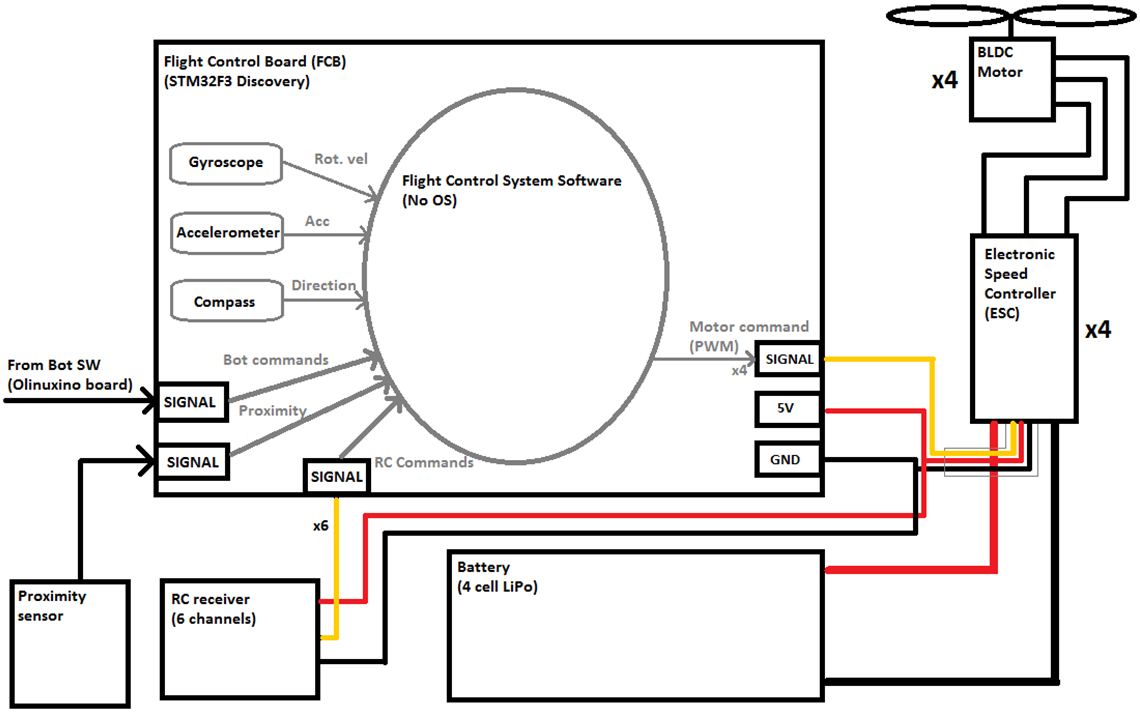
\includegraphics[scale=0.42]{images/fcb-sw-hw-design.png}
    \caption{FCB software architecture and circuit routing overview diagram. Red lines are $5$ $V$, black are ground and yellow are signals.}
    \label{fig:fcb-sw-hw-arch}
\end{figure}

	\section{Real-time Design}
\begin{figure}[h]
    \centering
    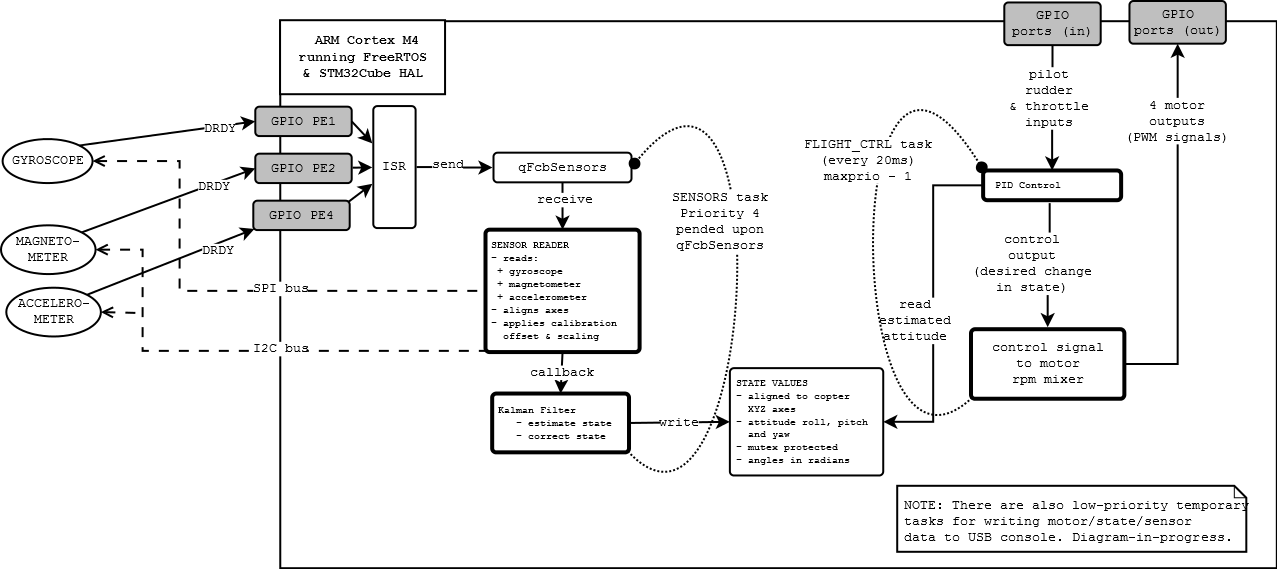
\includegraphics[width=\textwidth]{images/FcbThreadsOverview.png}
    \caption{FCB FreeRTOS threads \& queue diagram}
    \label{fig:freertos-threads-queues-diag}
\end{figure}

	\section{Code Documentation}

		\subsection{CMSIS}

		\subsection{STM32F3xx HAL Drivers}
STMicroelectronics provides an extensive library simplifying application interaction with the low-level registers of the MCU. These are known as the Hardware Abstraction Layer (HAL) Drivers, which are a part of the STM32Cube software development package. More detailed documentation on the HAL Drivers library can be found in \cite{stm32f3haldrivers}.

		\subsection{STM32 USB Device Drivers}

		\subsection{STM32F3Discovery Board-specific Package}

		\subsection{FreeRTOS}

		\subsection{FreeRTOS Plus CLI}

		\subsection{FCB Control}

		\subsection{FCB Communication}

		\subsection{FCB Sensors}

		\subsection{FCB Utilities}

		\subsection{NanoPB Protocol Buffer}

\begin{thebibliography}{99}
\bibitem[1]{stenberg} Model-based Design Development and Control of a Wind Resistant Multirotor UAV, C. Månsson, D. Stenberg, Dept. of Automatic Control LTH 2014, \url{http://www.control.lth.se/Publication/5947.html}
\bibitem[2]{bresciani} Modelling, Identification and Control of a Quadrotor Helicopter, T. Bresciani, Dept. of Automatic Control LTH 2008, http://\url{www.control.lth.se/Publication/5823.html}
\bibitem[3]{stm32f3discovery1} UM1562 User Manual: Getting started with software and firmware environments for the STM32F3DISCOVERY Kit, ST Microelectronics, \url{http://www.st.com/web/catalog/tools/FM116/SC959/SS1532/PF254044}
\bibitem[4]{stm32f303refman} RM0316 User Manual: Reference Manual for  STM32F303xB/C, STM32F303x6/8, STM32F328x8 and STM32F358xC advanced ARM®-based 32-bit MCUs, ST Microelectronics, \url{http://www.st.com/web/en/resource/technical/document/reference_manual/DM00043574.pdf}
\bibitem[5]{stm32f3discovery2}UM1570 User Manual: STM32F3DISCOVERY Discovery kit for STM32F303xx microcontrollers, ST Microelectronics, http://\url{www.st.com/web/catalog/tools/FM116/SC959/SS1532/PF254044}
\bibitem[6]{stm32f3progman}PM0214 Programming Manual: STM32F3 and STM32F4 Series Cortex®-M4 programming manual, ST Microelectronics, http://\url{www.st.com/st-web-ui/static/active/en/resource/technical/document/programming_manual/DM00046982.pdf}
\bibitem[6]{stm32f3haldrivers}UM1786 User Manual: Description of STM32F3xx HAL drivers, ST Microelectronics, http://\url{http://www.st.com/st-web-ui/static/active/en/resource/technical/document/user_manual/DM00122016.pdf}
\bibitem[7]{spektrumar610userguide}Spektrum AR610 User Guide, Spektrum 2012, \url{https://www.spektrumrc.com/ProdInfo/Files/SPMAR610_Manual_EN.pdf}

\end{thebibliography}

\end{document}                  % End of document
